\chapter{Deep-Learning-basierte Action Recognition}
\label{ch:sota}

Dieses Kapitel widmet sich dem aktuellen Forschungsstand im Bereich \gls{har}.
Der Hauptforschungsstrang in diesem Bereich beschäftigt sich mit Modellen, die anhand von generischen Datensets optimiert werden, die ein breiteres Spektrum an Anwendungsdomänen abdecken, als Sportarten, wie Fußball.
So soll sichergestellt werden, dass die Modelle besonders gut abstrahieren und sich in speziellen Domänen (hier Fußball) leicht nachtrainieren lassen (\gls{transfer-learning})~\cite{Burkov19}.
Daher werden im Folgenden Modelle mit allgemeingültiger Anwendbarkeit rekapituliert, die in einem späteren Schritt mit Daten aus der Fußballdomäne weiter abgestimmt werden.
\gls{har} gilt als der Kernproblem aufbauenden Probleme von Action Detection bis Video Understanding~\cite{Jiang19,Xia20}.
Auf diverse Möglichkeiten ungeschnittenen Videos zu verarbeiten oder die \gls{har} in eine zeitliche Action Detection zu integrieren wird gegen Ende des Kapitels eingegangen.

\section{Deep-Learning-Modelle zur Action Recognition}
\label{sec:deep-learning-modelle-zur-action-recognition}

Der Schlüssel zu einer guten \gls{har} ist die Erlernbarkeit von Bewegung (Motion).
Bewegung setzt sich zum einen aus der Erscheinung (appearance) von Objekten innerhalb stiller Frames und zum anderen aus der Dynamik (dynamics) entlang mehrere Frames zusammen~\cite{Sun15,Wang16}.

Die im Nachgang vorgestellten Kategorien haben unterschiedliche Ansätze diese beiden Faktoren zu erlernen und zu kombinieren.
In~\cite{Karpathy14} wurden erstmalig verschiedene Methoden verglichen, Bewegung in Videos einzufangen.
Dabei wurden die in \autoref{fig:fusion-types} gezeigten Ansätze Late-, Early und Slow-Fusion vorgestellt.
Allen drei liegt dasselbe 2D-CNN-Backbone zugrunde, welches einer abgewandelten Form von AlexNet entspricht.

\begin{figure}[h!]
    \centering
    \bigimage{img/03_Karpathy14}{0.8\textwidth}
    \caption{Fusion-Modelle für Frame-Features (Quelle:~\cite{Karpathy14})}
    \label{fig:fusion-types}
\end{figure}

In Late-Fusion-Modellen werden zunächst Features pro Frame erzeugt, wie es in einem 2D-\gls{cnn} der Fall ist und die fertigen Frame-Features werden erst in den allerhintersten Layern verknüpft.
Bei Slow-Fusion-Modellen fließen die Informationen aller Frames hingegen schon im ersten Layer ein.
Ein Kompromiss beider Anätze stellt die Slow Fusion dar, in der Features für je eine Untermenge der Frames verarbeitet und diese hierarchisch verknüpft werden.
Die drei Kategorien werden im weiteren Verlauf als Oberkategorien immer wieder aufgegriffen, während deren konkrete Umsetzung in~\cite{Karpathy14} unter dem Projektnamen DeepVideo referenziert wird.

%\autoref{fig:methods} zeigt einen Auszug konkreter Modelle, die unter diese drei Kategorien fallen und im weiteren Verlauf geneuer vorgestellt werden.

%\begin{figure}[htbp!]
%    \centering
%    \bigimage{fig/methods}{0.9\textwidth}
%    \caption{Lösungsansätze für das \gls{har}-Problem (Quelle: Eigene Darstellung)}
%    \label{fig:methods}
%\end{figure}

\subsection{Early Fusion}
\label{subsec:early-fusion}

Im Early-Fusion-Verfahren aus DeepVideo~\cite{Karpathy14} werden die drei Input-Kanäle (\gls{rgb}) aller Frames konkateniert und gleichwertig in das CNN-Backbone gegeben.
Erscheinung und Dynamik werden also parallel und von Anfang an erfasst.
Allerdings kann das Netz nicht unterscheiden, welche Kanäle zu welchem Frame gehören.
Somit herrscht keine Ordnung unter den Frames, \dh die Reihenfolge geht verloren.
Es kann keine echte Bewegung erkannt werden, sondern nur ein durchschnittliches Erscheinungsbild.
Das Öffnen einer Tür könnte \zB nicht von dem Schließen einer Tür unterschieden werden.
Ein weiterer Nachteil ist, dass sich mit dieser Methode nur wenige Frames zeitgleich verarbeiten lassen.

Im Slow-Fusion-Verfahren von DeepVideo~\cite{Karpathy14}, das eine hierarchische Form der Early Fusion darstellt, werden zunächst einzelne Frames in überlappende Intervalle gegliedert.
Diese werden dann, wie bei Early Fusion, als gleichwertige Kanäle verarbeitet.
Nach wenigen Schichten werden die Low-Level-Features erneut fusioniert.
Dennoch verliert das Modell die zeitlichen Informationen schließlich nach der letzten Fusion wieder~\cite{Tran15}.

Auch wenn keines dieser Modelle praktische Relevanz erlangte, zeigten die Experimente, dass Bewegung am besten lernbar ist, wenn Erscheinung- und Dynamik im gleichen Tempo erfasst wird.
Das Slow-Fusion-Modell schneidet entsprechend am besten ab.

\subsubsection{Two Stream Network}

Eine weitere Möglichkeit Bewegungsinformationen aus Videos zu extrahieren ist durch die Berechnung von Optischem Fluss.
Die Differenz zweier Bilder kann damit wieder als ein oder zwei (für horizontale und vertikale Bewegungen) neue Bilder gespeichert werden.

Das sogenannte Two Stream Network aus~\cite{Simonyan14} (siehe \autoref{fig:two-stream}) ist ein Modell, das mit zwei Input-Quellen in getrennten Netzen operiert.
Im ersten Stream (Spatial Stream) wird ein einzelner Frame als normales Farbbild in ein CNN-backbone gegeben.
Der zweite Stream (Temporal Stream) nimmt mehrere Bewegungsbilder pro \gls{clip}.
Dazu wird für alle Frames des \glspl{clip} vorab die Differenz als Optischer Fluss gespeichert.
Diese Bilder (je zwei pro Ausrichtung) werden als gleichwertige Kanäle in einen zweiten Stream gegeben.
Am Ende werden die Features aus beiden Streams mit einer \gls{svm} fusioniert.

Da die Frames auch hier als gleichwerige Kanäle behandelt werden, zählt es ebenso zu den Early-Fusion-Modellen und leidet daran, das keine Reihenfolgen abgebildet werden kann.
Dennoch erzielt es bessere Ergebnisse, da durch die Hinzunahme von Optischem Fluss externe Dynamik-Features hinzukommen.

Der wesentliche Unterschied zur Early Fusion in~\cite{Karpathy14} ist die getrennte Verarbeitung von Erscheinung und Dynamik in jeweils getrennten Netzen.
Motiviert ist diese Entscheidung durch die Two-Stream-Hypothese aus~\cite{Goodale92}, die besagt, dass der visuelle Kortex des menschlichen Gehirns Bewegung ebenfalls in zwei Strömen erfasst:
dem dorsalen Strom für die Erfassung von Dynamik und dem ventralen Strom für die Erkennung von Objekten.

Trotz langanhaltender Popularität ist der Einsatz von Optischem Fluss in Zusammenspiel mit Deep-Learning problematisch~\cite{Zhu17}:
Zum einen müssen die Differenz-Bilder vorab berechnet werden.
Das führt zu zusätzlichem Zeit- und Speicheraufwand, der mit der Anzahl von Frames skaliert und im Kontext dieser Arbeit nicht unerheblich ist.
Eine Echtzeit-Inferenz längerer \glspl{clip} ist mit gewöhnlicher Server-Hardware schon nicht möglich.
Des Weiteren sind die Modelle nicht Ende-zu-Ende trainierbar.
Die Inferenz besteht aus zwei getrennten Schritten: der Berechnung von Optischem Fluss und dem Training der Netze.
Der Optische Fluss selbst kann als Zwischenergebnis nicht mit-optimiert werden und ist damit nicht unbedingt auf die High-Level-Aufgabe zugeschnitten \cite{Zhu17}.

\begin{figure}
    \centering
    \begin{subfigure}[b]{.5\textwidth}
        \centering
        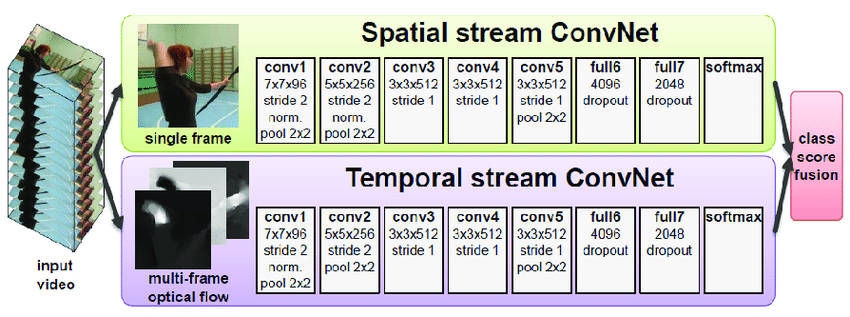
\includegraphics[width=.95\linewidth]{img/03_Simonyan14}
        \caption{Two Stream Network (Quelle:~\cite{Simonyan14})}
        \label{fig:two-stream}
    \end{subfigure}%
    \begin{subfigure}[b]{.5\textwidth}
        \centering
        \bigimage{img/03_Zhu17}{0.95\textwidth}
        \caption{Hidden Two Stream Network (Quelle:~\cite{Zhu17})}
        \label{fig:hidden-two-stream}
    \end{subfigure}
\end{figure}

\subsubsection{Hidden Two Stream Network}

Die genannten Probleme mit Optischem Fluss konnten schließlich mit dem Hidden Two Stream Network aus~\cite{Zhu17} überwunden werden.
\cite{Zhu17} beschreibt einen Ansatz, um beide der genannten Nachteile des Two-Stream-Modells zu kompensieren.
In der Arbeit wurde ein drittes zusätzliches Netz namens MotionNet trainiert, das aus zwei aufeinander folgenden Frames den resultierenden Optischen Fluss selbst generiert.
Das MotionNet wird dem Temporal Stream einfach vorgeschaltet (siehe \autoref{fig:hidden-two-stream}), sodass der Optische Fluss durch die Inferenz des MotionNets direkt errechnet wird und kein aufwendiges Pre-Processing notwendig ist.

Das Ergebnis ist eine bis zu zehnmal schnellere Verarbeitung bei fast gleichbleibender Genauigkeit.
Zudem kann die Erzeugung des Optischen Flusses während des Trainings an die spezielle Aufgabendomäne angepasst und optimiert werden.

\subsection{Late Fusion}
\label{subsec:late-fusion}

In Late-Fusion-Modellen werden die Frames eines \glspl{clip} zunächst nur einzeln in einem 2D-CNN-Backbone zu Frame-Features verarbeitet.
Dies entspricht im ersten Schritt einer Feature-Extraktion, die nur Erscheinungs-Features generiert.
Erst in einem zweiten Schritt wird die Dynamik anhand der Frame-Features erfasst und aggregiert.
Ein entscheidender Nachteil dieser Ansätze ist, dass in den vorderen Layern sehr viele redundante Informationen erhoben werden.
Ein weiterer Nachteil besteht darin, dass dynamische Features im Verhältnis deutlich unterrepräsentiert sind~\cite{Karpathy14}.
Die Feature-Aggregation erfolgt über Konkatenieren, Pooling oder den Einsatz eines \glspl{rnn}.

Die Aggregation in DeepVideo~\cite{Karpathy14} wird durch Konkatenation der Frame-Features gelöst.
Aus den Frames eines \glspl{clip} werden jeweils einzelne Features generiert.
Diese werden alle zu einem langen Vektor konkateniert und abschließend in einem \fc-Layer klassifiziert.
So wird Dynamik durch die Differenz der jeweiligen Frame-Features abgebildet.

\subsubsection{Conv Pooling}

Eine weitere Option Frame-Features zu aggregieren ist durch Pooling.
Dabei werden die Frame-Features vor dem ersten \fc-Layer zu einem 3D-Volume gestapelt und mit einem oder mehreren \pool- und einem \fc-Layer klassifiziert.

In~\cite{Ng15} wurden verschiedene Varianten zur Erfassung von Bewegung getestet.
Die Frame-Features (generiert durch InceptionV1-Backbone) wurden mit einem Max-Pooling-, zwei \fc- und einem Softmax-Layer weiterverarbeitet.
Das Pooling beschränkt sich auf die zeitliche Dimension (Temporal Pooling), sodass die räumliche Dimension komplett erhalten bleibt.
In der zeitlichen Dimension spielt die Reihenfolge allerdings immer noch keine Rolle, da jeweils nur nach Maxima gepoolt wird~\cite{Carreira17}.
Die Klassifikation findet letztlich auf Basis hervorstechender Regionen innerhalb der Frame-Features statt.

%\begin{figure}[h!]
%    \centering
%    \bigimage{img/03_Ng15_conv_pooling}{0.3\textwidth}
%    \caption{Conv Pooling}
%    \label{fig:conv-pooling}
%\end{figure}

Ein technischer Vorteil dieser Architektur ist allerdings, dass sie mit beliebig vielen Frames funktioniert, da das \pool-Layer einen variablen tiefen Input verarbeiten kann.
Das macht das Modell vergleichsweise leichtgewichtig, denn die Zahl der Parameter ist unabhängig von der Zahl der Frames.
Da die Feature-Extraktion viele redundante Informationen für konsekutive Frames berechnet, reicht in diesem Verfahren auch eine niedrigere Subsamplingrate von 6 \gls{fps}.

\subsubsection{Two-Stream-Fusion}

Um den Fortschritt des seinerzeit populären Two-Stream-Modells mit Conv Pooling zu verbinden, stellte~\cite{Feichtenhofer16} 2016 die sogenannte Two Stream Fusion vor.
Das Verfahren unterscheidet sich wesentlich dadurch, dass die Ströme nicht nur am Ende, sondern schon in früheren Layern fusioniert werden.
Im Vergleich zum Conv Pooling wird jedoch kein Temporal Pooling genutzt, sondern ein 3D-Pooling (siehe \autoref{fig:two-stream-fusion}), das sowohl die zeitliche als auch die räumliche Dimension des Frame-Feature-Volumes reduziert.

Die zwei Ströme aus dem Vorgängermodell (spatial-, temporal stream) werden transformiert zu zwei neuen Strömen:
Zunächst findet nach dem fünften \conv-Layer eine Fusion statt.
Als Input werden die Feature-Maps beider Streams abwechselnd zu einer neuen Feature-Map gestapelt und mittels 3D-Faltung gefolgt von 3D-Pooling fusioniert.
Das Ergebnis ist der sogenannte Spatiotemporal Stream, der den alten Spatial Stream ersetzt.
Parallel findet im weiter fortlaufenden Temporal Stream ebenfalls ein 3D-Pooling statt, sodass beide Streams die gleiche Auflösung aufweisen.
Später wird der alter Temporal Stream nach dem letzten \fc-Layer erneut mit dem Spatiotemporal Stream fusioniert.

Die Fusionen bieten erstmalig eine Pixel-weise Kombination beider Streams.
So kann \zB das räumliche Frame-Feature eines erkannten Balls mit dem dynamischen Feature einer Flugkurve pixelgenau kombiniert werden.

Ein Nachteil dieser Architektur ist wiederum, dass Bewegung auf zweierlei Mittel zurückgeführt werden kann.
Durch den Einsatz von Optischem Fluss in mehreren Kanälen und durch die neuartigen Fusion-Layer.
Das Lernen redundanter Informationen kann die Performance so letztlich ausbremsen.

\begin{figure}
    \centering
    \begin{subfigure}[b]{.5\textwidth}
        \centering
        \bigimage{img/03_Feichtenhofer16}{0.95\textwidth}
        \caption{Architektur: TwoStream Fusion (Quelle:~\cite{Feichtenhofer16})}
        \label{fig:two-stream-fusion}
    \end{subfigure}%
    \begin{subfigure}[b]{.5\textwidth}
        \centering
        \bigimage{img/03_Girdhar17}{0.95\textwidth}
        \caption{Architektur: ActionVLAD (Quelle:~\cite{Girdhar17})}
        \label{fig:avlad}
    \end{subfigure}
\end{figure}

\subsubsection{Action VLAD}

Ein weiterer Ansatz ist die Klassifikation basierend auf einem Feature-Extraktor wie in~\cite{Girdhar17}.
Das Modell ActionVLAD gilt als eine Erweiterung des Conv Pooling, wobei Features nicht aus dünn gesampleten Frames, sondern aus allen Frames des \glspl{clip} extrahiert werden.
Die Aggregation findet ebenfalls nach dem letzten \conv-Layer eines VGG-16-Backbones statt.

Statt eines Max-Pooling-Layers wird allerdings ein \gls{bovw}-Verfahren ~\cite{Zisserman03} eingesetzt (siehe \autoref{fig:avlad}).
Die aggregierten Features werden auf ein Vokabular von Action Words (in 64 Cluster) projiziert.
Diese Cluster repräsentieren die typischen (Sub-)Aktionen aus denen sich die eigentlichen Klassen herausbilden~\cite{Ghosh18}.
Jeder Frame wird schließlich auf ein Cluster projiziert, sodass sich für den gesamten \gls{clip} ein Feature-Vektor mit je der Anzahl an Treffern pro Cluster ergibt.
Dieser Feature-Vektor wird mithilfe eines weiteren Klassifizierers dann auf die finale Klasse projiziert.
Alle Parameters, darunter die Action Words, sowie die Feature-Extractors werden während des Trainings des eigentlichen Klassifizierers mitgelernt.

Zusätzlich gibt es auch eine Version, die ActionVLAD in die Two Stream Architektur integriert.
Die Features werden hier jedoch wieder separat pro Strom berechnet und erst am Ende kombiniert, in dem der Durchschnitt beider Vektoren genommen wird.

\subsubsection{Feature-Aggregation mit RNNs}

Die dritte Möglichkeit Frame-Features zu aggregieren ist der nachgelagerte Einsatz eines \gls{rnn}.
Die Folge einzelner Frame-Features kann somit als Zeitreihe angesehen werden, die in ihrer ursprünglichen Reihenfolge verarbeitet wird.

In~\cite{Donahue14} wurde erstmalig das Long-term Recurrent Convolutional Networks (LRCN) vorgestellt.
Dort werden je Frame visuelle Features mit einem auf AlexNet basierenden Backbone extrahiert.
Die Frame-Features werden dann nach und nach in ein LSTM-Layer geleitet (siehe \autoref{fig:lrcn}).
Die Klassifizierung eines \glspl{clip} setzt sich schließlich aus dem Durchschnitt aller Outputs $y_{t_i}$ zusammen.

\begin{figure}[h!]
    \centering
    \bigimage{img/03_Donahue14}{0.4\textwidth}
    \caption{Architektur: LRCN (Quelle:~\cite{Donahue14})}
    \label{fig:lrcn}
\end{figure}

Herausfordernd ist hierbei, dass die visuellen Frame-Features genug relevante Informationen für das abschließende LSTM-Layer behalten.
Das Modell wurde jeweils mit RGB-Bildern und Optischem Fluss getestet, wobei die Variante mit Optischem Fluss wesentlich bessere Ergebnisse erzielt.
Dies ist \ua ein Hinweis darauf, dass die Bewegung in den ursprünglichen Bildern erst zu spät erfasst wird.
Das Modell hat ebenfalls eine variable Input-Länge, ist aber deutlich schwerer zu trainieren, da die Backpropagation über alle Frames geschieht und so sehr anfällig für Overfitting ist.

In~\cite{Ng15} wurde neben dem bereits erwähnten Conv Pooling auch ein Modell vorgestellt, das Frame-Features mit einem mehrschichtiges LSTM aggregiert.
Im Gegensatz zum LRCN werden fünf LSTM-Schichten mit je 512 Memory-Zellen statt nur einer Schicht gewählt und das 2D-CNN-Backbone entspricht InceptionV1.
Auch im Training gibt es einen gravierenden Unterschied:
während bei LRCN ein Backpropagation-Schritt pro \gls{clip} (mit $T = 16$ Frames) gemacht wird, wird er in diesem Modell pro Frame (bei $T = 30$) gemacht.

\subsection{3D-Convolution}
\label{subsec:3d-conv}

Die nächste große Generation der \gls{har}-Modelle war die erstmalig in~\cite{Ji13} vorgestellte 3D-Faltung (3D-Convolution).
Die 3D-Faltung funktioniert analog zur 2D-Faltung aus \autoref{sec:cnn}:
Statt eines $(C \times S^2)$-Inputs, erhält das Netz einen $(C \times T \times S^2)$-Input.
Alle \conv- und \pool-Layer haben nun dreidimensionale Kernel und erzeugen vierdimensionale Feature-Maps.

Im Gegensatz zu vorherigen Early-Fusion-Modellen werden zeitliche Informationen nicht gemittelt.
Die zeitliche Ordnung der Frames bleibt also erhalten.
Außerdem werden sie, anders als bei Late Fusion, stets im gleichen Tempo erhoben und kombiniert.
3D-CNNs haben allerdings auch wesentlich mehr Parameter und \gls{flops} als alle zuvor vorgestellten Modelle~\cite{Zhu19}~\cite{Carreira17}.

\subsubsection*{C3D (Convolution 3D)}

C3D~\cite{Tran15} ist das erste 3D-CNN, das an großen \gls{har}-Datensets getestet wurde.
Seinerzeit war es als Feature Extractor konzipiert, der $T=16$ Input-Frames zu einem 4096-Elemente-langen Feature-Vektor komprimiert.
Zur Klassifikation wurde anschließend eine \gls{svm} eingesetzt, wobei auch eine direkte Klassifikation im letzten \fc-Layer möglich ist.
Das Netz basiert auf keinem vorhergegangenen Backbone, hat eine Tiefe von insgesamt 10 Schichten (davon 8 3D-\conv-Layer) und verarbeitet \glspl{clip} mit einer Auflösung von $S=112$ Pixeln.
In jedem Layer wird ein $(3 \times 3 \times 3)$-Kernel, gefolgt von einem $(2 \times 2 \times 2)$-\pool-Layer verwendet.
Entscheidende Vorteile sind eine generische Feature-Extraktion und die kompakte Repräsentation.

Bei seiner Vielzahl an Parametern gestaltet es sich allerdings schwierig das Netz von Grund auf neu zu trainieren.
Ebenfalls problematisch ist die Beschränkung auf $T=16$ Frames.
So muss für längere \glspl{clip} stets der Durchschnitt einzelner Chunks erfasst werden, was mit zusätzlichen Ungenauigkeiten einhergeht.

\begin{figure}[h!]
    \centering
    \bigimage{img/03_Varol16}{0.9\textwidth}
    \caption{Architektur: LTC (Quelle:~\cite{Varol18})}
    \label{fig:ltc}
\end{figure}

\subsubsection*{LTC (Long-term Temporal Convolution)}

Letzteres Problem sollte durch die Veröffentlichung von LTC~\cite{Varol18} behoben werden.
Das Modell unterstützt mit $T=100$ Frames deutlich längere \glspl{clip}, kompensiert dies aber mit einer deutlich geringeren Auflösung von $S=71$ Pixeln.
Ansonsten ähnelt die Architektur (in \autoref{fig:ltc}) der von C3D mit der Ausnahme, dass ausschließlich $(3 \times 3 \times 3)$-Kernel verwendet wurden.

\subsubsection*{I3D (Inflated 3D ConvNet)}

Mit I3D~\cite{Carreira17} wurde das erste 3D-CNN veröffentlicht, das eine Transfer-Learning-Technik nutzt um bestehende Features eines 2D-CNNs wiederzuverwenden.
I3D basiert auf der Architektur von InceptionV1, die um eine dritte Dimension aufgeblasen (inflated) wird.
Beim Prozess der \emph{Inflation} wird jeder bereits vortrainierte 2D-Kernel um eine dritte Dimension erweitert, indem die vortrainierten Gewichte entlang der zeitlichen Achse kopiert werden.
\Dh das Netz ist danach vortrainiert für die Klassifizierung stiller Videos \bzw Standbilder.

%\begin{figure}[h!]
%    \centering
%    \bigimage{img/03_Carreira17}{0.95\textwidth}
%    \caption{Architektur: I3D (Quelle:~\cite{Carreira17})}
%    \label{fig:i3d}
%\end{figure}

Der Größenunterschied zu C3D und LTC spiegelt sich zwar in der Tiefe des Netzes wider, dennoch hat I3D deutlich weniger Parameter aufgrund der effizienten Inception-Architektur und kann somit deutlich schneller trainiert werden.
\glspl{clip} können mit je $T=64$ Frames inferiert werden.

\subsubsection*{T3D (Temporal 3D)}

T3D~\cite{Diba17} ist analog zu I3D eine 3D-Variante von DenseNet.
Die Besonderheit ist hierbei die Hinzunahme eines neuartigen modularen Block-Typen zur Erfassung dynamischer Features von variabler Dauer.

Bei der gewöhnlichen 3D-Faltung wird stets eine lokale Nachbarschaft des jeweiligen Pixels betrachtet, welches im Mittelpunkt der Faltung steht.
Die hier neuen TTLs (Temporal Transition Layer) erfassen allerdings zeitgleich Bewegungen verschieden langer Zeiträume.
Kurze Bewegungen werden durch einen Kernel mit einer vergleichsweise geringen zeitlichen Dimension (flache Kernel) eingefangen und lange Bewegungen mit einem deutlich tieferen Kernel.
In jedem TTL operieren drei verschiedene Kernel, deren Output zu einer neuen Feature-Map konkateniert und gepoolt wird.
Das Netz kann mit einem flachen Kernel \zB eine kurze Geste des Schiedsrichters einfangen und gleichzeitig mit einem tieferen Kernel den Ball verfolgen, der langsam ins Aus rollt.
Da die räumliche Auflösung innerhalb des TTL stets gleich ist, können die Features pro Kernel anschließend Pixel-genau kombiniert werden.
Die Gesamtarchitektur, sowie die eingesetzten TTLs sind in \autoref{fig:t3d} abgebildet.

\begin{figure}
    \centering
    \begin{subfigure}[b]{.5\textwidth}
        \centering
        \bigimage{img/03_Diba17}{\textwidth}
        \caption{Architektur: T3D (Quelle:~\cite{Diba17})}
        \label{fig:t3d}
    \end{subfigure}%
    \begin{subfigure}[b]{.5\textwidth}
        \centering
        %\bigimage{img/03_Girdhar17}{0.95\textwidth}
        \caption{Schaubild: Non-Local-Blöcke (Quelle:~\cite{Wang18})}
        \label{fig:non-local}
    \end{subfigure}
\end{figure}

\subsubsection*{Non-Local Networks}

Die in~\cite{Wang18} vorgestellten Non-Local Networks haben eine ähnliche Absicht, wie die TTLs in T3D.
Analog zu TTLs wurden Non-Local-Blöcke entwickelt, die direkte Verbindungen zwischen entfernten Pixeln abbilden können -- mit dem Unterschied, dass keine zusätzliche Faltung benötigt wird.
Sie transformieren die Feature-Maps eines 3D-CNNs in jedem Pixelwert $i$ wie in \autoref{eq:non-local}:

\begin{equation}
\label{eq:non-local}
\begin{split}
    y_i             & = \sum_{\forall j} f_p(x_i, x_j) g(x_j) \\
    f_p(x_i, x_j)   & = softmax(x_i^T W^T_\theta W_\phi x_j) \\
    g(x)            & = W_g x
%y_i             & = \frac{1}{\sum\limits_{\forall j}f(x_i, x_j)} \sum\limits_{\forall j} f_p(x_i, x_j) W_g x_j \\
%f_p(x_i, x_j)   & = e^{W_{\theta} x_i^T W_{\phi} x_j}
\end{split}
\end{equation}

Die Funktion $f_p$ ist eine paarweise Funktion, die die Ähnlichkeit zweier Pixel ausdrückt und entspricht hier der Embedded-Gaussian-Funktion.
$g(x)$ verknüpft jedes Pixel mit der Gewichtsmatrix $W_g$, die für die jeweilige Aufgabe optimiert werden muss.
$W_\theta$ und $W_\phi$ ergeben sich wiederum aus der punktweisen $(1 \times 1 \times 1)$-Faltung eines Pixels.

Non-Local-Blöcke können nicht-lokale Beziehungen direkt abbilden, indem die Interaktion zwischen allen Pixeln des Input-Volumes berechnet werden (siehe \autoref{fig:non-local}).
Das hat zur Folge, dass insbesondere schnelle Bewegungen besser eingefangen werden können als es durch reine 3D-Faltung möglich ist.
Verglichen mit den verschieden tiefen Filtern in TTLs, müssen hier keine diskreten Grenzen (für die zeitliche Dimension der TTL-Kernel) gezogen werden.
Die Blöcke haben vielmehr die Mächtigkeit Bewegungen jedmöglicher Dauer implizit abzubilden.

Durch den Einsatz eines Non-Local-Blocks bleibt zudem die Größe der Feature-Map erhalten, sodass sie sich an beliebigen Stellen eines 3D-CNNs einfügen lassen.
Die Experimente, in denen Non-Local-Blöcke an verschiedenen Stellen eines I3D-Netzes (NL-I3D) getestet wurden, zeigen, dass schon wenige (\zB 5) Non-Local-Blöcke reichen um genauere Ergebnisse zu erzielen.

\subsubsection*{SlowFast}

Zuletzt wurde in~\cite{Feichtenhofer18} SlowFast vorgestellt -- ein Modell basierend auf einem 3D-ResNet, welches kurze und lange Bewegungen durch eine Architekturänderung separate erfasst und kombiniert.
In SlowFast wird Bewegung durch ein Netz aus zwei Strömen erfasst.
Die beiden Ströme sind wie folgt konzipiert:

\begin{description}
    \item[Slow pathway]
    (langsamer Strang) fokussiert sich auf räumliche Features, indem ein \gls{clip} mit einer niedrigen Framerate gesamplet wird.
    Aufgrund der niedrigen Framerate können nur wenig redundante Informationen gesammelt werden.
    Dies wird zusätzlich gehemmt, indem die Hälfte der Residual-Blöcke nur mit 2D-Faltungen operieren.
    \item[Fast pathway]
    (schneller Strang) generiert räumliche Features, indem ein \gls{clip} mit einer höheren Framerate gesamplet wird und wenige Kanäle zur Verfügung stehen.
    So wird ihm die Möglichkeit genommen sich räumliches zu fokussieren.
    Stattdessen muss er sich implizit auf die Dynamik zwischen den Frames fokussieren.
\end{description}

\begin{figure}[h!]
    \centering
    \bigimage{img/03_Feichtenhofer18}{0.8\textwidth}
    \caption{Architektur: SlowFast (Quelle:~\cite{Feichtenhofer18})}
    \label{fig:slowfast}
\end{figure}

An zwei Stellen im Netz werden die dynamischen Features vom schnellen Strang in den langsamen Strang fusioniert.
Diese Verbindungen werden als Lateral Connection bezeichnet und ähneln dem Vorgehen in der 3D-Fusion~\cite{Feichtenhofer16}.
Schließlich werden die Features beider Stränge je mit einem Avg-\pool-Layer auf eine fixe Länge gestaucht und konkateniert.
Ein abschließendes \fc-Layer dient zur Klassifikation.
Die Gesamtarchitektur ist in \autoref{fig:slowfast} zu sehen.

Das Vorgehen ist motiviert durch die Funktionsweise Retinaler Ganglienzelle im menschlichen Auge.
Dort operieren P-Zellen (\emph{P} für parvozellulär) mit einer geringeren Frequenz als M-Zellen (\emph{M} für magnozellulär).
Das Verhältnis von P- und M-Zellen ist etwa 4:1.
Genau dieses Verhältnis wurde auch in der Architektur abgebildet, indem der Slow Pathway 80 \% aller Parameter beansprucht.

Durch das dynamische Avg-Pooling am Ende ist die Summe aller Parameter unabhängig von der \gls{clip}-Länge (nicht aber die Größe der Feature-Map).
Es ist derart implementiert, dass die \conv-Features auf eine fix definierte Zielauflösung komprimiert werden, sodass theoretisch ein Training mit beliebig hoher Auflösung $T \times S^2$ möglich ist.

Ein entscheidender Hyperparameter ist die Wahl von $\alpha$, dem temporären Stride des Slow Pathways.
Die Wahl von $\alpha$ führt dazu, dass immer nur einer von $\alpha$ Frames gesamplet wird.
Getestet wurden verschiedene Varianten mit $\alpha = 8$ und $\alpha = 16$, basierend auf ResNet-50 und ResNet-101, sowie unter optionaler Hinzunahme von Non-Local-Blöcken.

\subsection{Factorized Convolution}
\label{subsec:factorized-convolution}

Spätestens mit der Veröffentlichung von I3D galt 3D-Faltung als der neue State of the art.
Aufgrund der Vielzahl an Parametern waren diese Modelle allerdings noch immer für viele Bereiche zu groß und zu schwer zu trainieren.
Infolgedessen wurden viele Ansätze publiziert, die versuchten die Idee von dreidimensionaler Faltung zu approximieren und dabei annähernd gute Ergebnisse mit weniger Parametern und Rechenoperationen zu ermöglichen.
Man spricht in diesem Zusammenhang von einer Faktorisierung der gewöhnlichen 3D-Faltung, die durch Architekturänderungen, die Einführung neuartiger Block-Typen oder durch die Anwendung von Group Convolution erfolgt.

\subsubsection{Faktorisierte Architektur}

In~\cite{Sun15} wird mit FstCN (Factorized spatio-temporal convolutional network) versucht 3D-Faltung in räumliche 2D-Faltung gefolgt von einer 2D-Faltung über die Zeit- und Kanaldimension, zu ersetzen.
Die Frames werden zunächst einzeln verarbeitet, sodass man ${T}$ 3D-Feature-Maps $(C \times S_x \times S_y)$ erhält.
Nach der normalen 2D-Faltung wird ein 4D-Tensor $(T \times C \times S_x \times S_y)$ aus allen Feature-Maps generiert und so transformiert, dass eine Feature-Map $(S_x * S_y \times T \times C)$ entsteht.
Es entsteht also ein Volume, welches in seinem Querschnitt ein Bild pro Pixel enthält.
Die Pixelwerte ergeben sich aus dem jeweiligen Kanal der Feature-Map und dem Frame-Index.
Diese Bilder werden nun analog mit 2D-Faltung weiter verarbeitet.

Zu beachten ist, dass die komplette Architektur durch Matrixtransformationen und 2D-Faltung faktorisiert wird.
Dieser Teil findet allerdings erst in den hinteren Layern des Netzes statt, womit es weiter zu den Late Fusion Modellen zählt.
Die Architektur hat zudem den Nachteil, dass Bewegungen nur über den gesamten Zeitkontext des \glspl{clip} erfasst werden können.
Kurze Bewegung oder Kombinationen von kurzen Bewegungen sind somit schwieriger abzubilden.

\subsubsection{Faktorisierte \conv-Blöcke}


Statt 3D-Faltung, wie bei FstCN, einmalig durch eine globale Architekturänderung zu faktorisieren, wurden in späteren Publikationen Ansätze entwickelt, die eine blockweise Faktorisierung an zahlreichen Stellen der Gesamtarchitektur einbinden.

Das erste relevante Modell dieser Kategorie ist P3D (Pseudo-3D Residual Net)~\cite{Qiu17}, deren Grundlage ein 3D-ResNet-Backbone ist.
In dem Netz wird jeder einzelne \res-Block faktorisiert, indem die bestehenden 3D-Kernel $(T \times S_x \times S_y)$ durch die Abfolge eines räumlichen $(1 \times S_x \times S_y)$- und eines zeitlichen $(T \times 1 \times 1)$-Kernels ersetzt wird.
Das Netz erfasst somit iterativ mit Wechsel erst räumliche und dann zeitliche Features.

Weiter werden drei der in \autoref{fig:p3d} gezeigten Blocktypen eingeführt und jeder bestehende \res-Block wird durch die Abfolge aller drei Blocktypen hintereinander ersetzt.

\begin{figure}[h!]
    \centering
    \bigimage{img/03_Qiu17}{0.45\textwidth}
    \caption{P3D-Blöcke}
    \label{fig:p3d}
\end{figure}

P3D ist nicht nur deutliche schlanker als vorherige 3D-CNNs.
Durch die Einführung zusätzlicher ReLu-Aktivierungen zwischen den 2D- und 1D-\conv-Layern entsteht auch doppelt so viel Nichtlinearität als zuvor.
Das Netz ist damit deutlich einfacher zu optimieren und kann komplexere Funktionen abbilden~\cite{Tran18}.

In~\cite{Tran18} wurden die Erfolge von P3D erneut aufgegriffen und im Zuge des Modells R2+1D verbessert.
Auch hier werden die \res-Blöcke jeweils durch 2D- gefolgt von 1D-\conv-Layern ersetzt.
Im Vordergrund steht hierbei allerdings die direkte Vergleichbarkeit mit 3D-Faltung indem, verglichen mit einem 3D-ResNet, die gleiche Zahl an Parametern verwendet wird.

Topologisch unterscheidet sich R2+1D von P3D durch den konsequenten Einsatz eines \res-Blocktypen, der dem Typ A aus \autoref{fig:p3d} entspricht.
Zusätzlich werden keine Bottlenecks verwendet und das Netz kann mit einer variablen Input-Länge aufgerufen werden, indem vor dem ersten \fc-Layer ein dynamisches Avg-\pool-Layer eingeführt wird, dass die Dimension der Feature-Map auf eine feste Tiefe reduziert (analog zu SlowFast) .

\subsubsection{Faktorisierung durch Group Convolution}

Die in \autoref{subsec:group-conv} bereits vorgestellte Group Convolution stellt ebenfalls eine Form von Faktorisierung (und zwar der Kanal-Interaktion) dar.

In~\cite{Tran19} wurden CSNs (Channel-Separated Convolutional Networks) vorgestellt.
CSNs basieren ebenfalls auf einem 3D-ResNet, benutzen jedoch Group Convolution.
Für eine 4-dimensionale Feature-Map, ersetzt die Faktorisierung nun die normale 3D-Faltung durch eine punktweise Faltung mit Kernel $(1, 1, 1)$ über alle Feature-Maps und eine Group Convolution mit Kernel $(3, 3, 3)$ pro Kanal.
Erstere sorgt für Interaktion zwischen den Kanälen innerhalb eines Pixels.
Letztere berechnet für einen einzelnen Index der Feature-Map die zeit-räumlichen Features.

Präsentiert wurden in diesem Zuge zwei verschiedene Modelle:
\begin{description}
    \item[interaction-preserved (ip-CSN)] Die $3 \times 3 \times 3$-\conv-Layer werden durch punktweise Faltung, gefolgt von Depthwise Convolution ersetzt.
    \item[interaction-reduced (ir-CSN)]  Die $3 \times 3 \times 3$-\conv-Layer werden nur durch Depthwise Convolution ersetzt.
    Alleine durch die Bottleneck-Blöcke der ResNet-Architektur kann noch Kanal-Interaktion hergestellt werden.
\end{description}

Ein noch globalerer Ansatz wird in~\cite{Feichtenhofer20} mit X3D (Expand 3D) präsentiert.
Grundlage ist eine 2D-Variante des Slow Pathway aus SlowFast, der ebenfalls Group-Convolution, wie in ip-CSN nutzt.
Die Basisarchitektur wird auf Basis verschiedener Faktoren schrittweise in eine dreidimensionale Variante expandiert:
Neben der raum-zeitlichen Dimension, wird auch die Dichte der gesampleten Frames (Framerate), die Anzahl der Kanäle innerhalb der Layer und die Anzahl der Layer selbst variiert.
Folgende Faktoren (siehe~\autoref{fig:x3d}) wurden mithilfe eines Coordinate Descent Algorithmus~\cite{Wright15} optimiert, um die finale Architektur zu bestimmen:

\begin{description}
    \item[$\gamma_s$] Faktor für höhere Auflösung ($\gamma_s = 1$ entspricht 112 Pixeln)
    \item[$\gamma_t$] Faktor für zusätzliche Frames ($\gamma_t = 1$ entspricht einem einzelnen Frame)
    \item[$\gls{tld:gamma-tau}$] Faktor für Subsampling: Nur jeder $\gamma_\tau$-te Frame wird gesamplet. ($\gamma_\tau = 1$ entspricht der Original-Framerate)
    \item[$\gamma_w$] Faktor für zusätzliche Residual-Blöcke innerhalb der vier \res-Layer der ResNet-Architektur ($\gamma_d = 1$ entspricht 1, 2, 5 und 3 Blöcken).
    \item[$\gamma_w$] Faktor für zusätzliche Kanäle pro Layer
    \item[$\gamma_b$] Faktor für zusätzliche Kanäle -- exklusiv für Bottleneck-Layer innerhalb der \res-Blöcke
\end{description}

\begin{figure}[h!]
    \centering
    \bigimage{img/03_Feichtenhofer20}{0.8\textwidth}
    \caption{Expansionsfaktoren in X3D (Quelle:~\cite{Feichtenhofer20})}
    \label{fig:x3d}
\end{figure}

In mehreren Phasen wurden die einzelnen Parameter jeweils um einen maximalen Faktor vergrößert.
Die Maximalwerte ergeben sich aus der in \gls{flops} gemessenen Komplexität der Gesamt-Architektur, die pro Phase durch das Doppelte der vorherigen Phase gedeckelt wird.
Für jeden Parameter wird die Änderungen durch den jeweils maximierten Faktoren getestet und der beste Faktor wird in die nächste Phase übernommen.
Dieser Prozess wurde insgesamt 13 mal wiederholt, wodurch sechs Versionen (X3D-XS bis X3D-XXL) der Architektur entstanden -- darunter:

\begin{description}
    \item[X3D-S] Alle Parameter bis auf $\gamma_w$ wurden in den ersten 7 Iterationen erhöht ($\gamma_t$ und $\gamma_\tau$ davon zweimal).
    Das Modell samplet $T=13$ mal jeden sechsten Frame bei einer Auflösung von $S=160$ Pixeln.
    \item[X3D-XL] Nach der zehnten Iteration steht ein Modell das jeden fünften Frame $T=16$ mal bei einer Auflösung von $S=312$ Pixeln samplet.
\end{description}

Die Ergebnisse zeigen zum einen, dass mehrere Sekunden langes Videomaterial auch mit wenigen Frames und einem dünnen Sampling verarbeitet werden kann.
Zum anderen sind besonders die Modelle (M bis XXL) interessant, da sie eine deutlich höhere Auflösung $S$ in Kombination mit deutlich weniger Kanälen als vorherige Modelle aufweisen und dabei zum Teil auch bessere Ergebnisse erzielen.
Vor allem aber sticht die geringe Zahl an Parametern hervor, die mit keiner der vorherigen Faktorisierungsmethoden vergleichbar ist.

%Zu beachten ist, dass alle zeitlichen Informationen bis zum finalen globalen \pool-Layer pro Kanal gewahrt werden.

\section{Long-term Aggregation Frameworks}
\label{sec:long-term-aggregation-frameworks}

Die meisten der vorgestellten Modelle können nur \glspl{clip} einer fixen oder zumindest begrenzten Länge klassifizieren.
Dieser Rahmen liegt je nach Modell zwischen 16 und 64 Frames.

Einige Modelle (darunter R2+1D, CSN, SlowFast und X3D) ermöglichen durch den Einsatz eines dynamischen Avg-\pool-Layers eine Variable Input-Länge.
Allerdings ist die Nutzung nur dann optimal, wenn die Modelle zuvor auch mit der gleichen Länge an Frames trainiert wurden.
Problematisch ist auch, dass die Feature-Maps proportional zur Input-Länge mitwachsen.
So wird das ohnehin speicherintensive Training noch schwieriger.

Eine weitere Möglichkeit, die aber ebenfalls nur im geringen Maße praktikabel ist, ist ein vorgelagertes Subsampling der \glspl{clip} (\cite{Ng15}).
Einige Modelle, wie X3D, nutzen ohnehin ein dünnes Sampling und nicht jeden Frame.
Werden die Frames allerdings zu dünn gesamplet, kann insbesondere bei 3D-\glspl{cnn} die Performance einbrechen, da konsekutive Frames zu unterschiedlich sind und die Kernel keine Zusammenhänge mehr herstellen können.

Benötigt der Classifier einen deutlich längeren Zeitkontext, als das trainierte Modell abbildet, sind weder das dynamische Avg-Pooling noch Subsampling ausreichend.
Stattdessen kann auf spezielle Long-term Aggregation Frameworks zurückgegriffen werden.

Ein besonders populäres Framework ist das TSN (Temporal Segments Network)~\cite{Wang16}~\cite{Wang19}.
Es bettet das eigentliche \gls{har}-Modell in einen spezielles Trainingssetup (siehe \autoref{fig:tsn}) ein.
TSN unterteilt den \gls{clip} zunächst in Unter-Segmente (genannt Snippets).
Innerhalb dieser Snippets wird jeweils ein Intervall zufallsbasiert bestimmt, dessen Länge in das entsprechend vortrainierte \gls{har}-Modell passt.
Diese Snippets werden nun wie gewohnt inferiert, sodass man den Feature-Vektor des letzten \fc-Layers erhält.
Für jeden Vektor wird der Fehler pro Klasse berechnet und über die Snippets gemittelt.
Darüber wird abschließend die Aktivierung berechnet, die zur Klassifizierung dient.

\begin{figure}[h!]
    \centering
    \bigimage{img/03_Wang19}{0.9\textwidth}
    \caption{Architektur: TSN (Quelle:~\cite{Wang19})}
    \label{fig:tsn}
\end{figure}

Die Architektur ist differenzierbar und wird optimiert mit dem über alle Segmente aggregiertem Output.
Somit können die Modellparameter anhand mehrere Snippets optimiert werden.
In der ursprünglichen Form wurde TSN mit dem Two Stream Modell genutzt.
Technisch gesehen lässt sich allerdings jedes der genannten Modelle einbinden~\cite{Kothawade19}.

Alternativ zu TSN kann das jeweilige \gls{har}-Backbone durch ein- oder mehrere \gls{rnn}-Layer erweitert werden.
Exemplarisch wird hier FASTER (Feature Aggregation for Spatio-temporal Redundancy)~\cite{Zhu19} erwähnt.
Durch FASTER soll nicht nur eine zeitliche Struktur über einen längeren Kontext abgebildet werden.
Zusätzlich soll vermieden werden, dass redundante Informationen erhoben werden.

Die Features des letzten \conv-Layers des CNN werden durch ein Avg-\pool-Layer geleitet.
Diese Features werden dann als Input des RNNs verarbeitet und haben Einfluss auf den Hidden State des RNNs.
Um das Modell zu beschleunigen werden statt eines Backbone-Modells zwei verschiedene Versionen verwendet, wobei beide vom gleichen Typ, aber mit unterschiedlicher Tiefe sind (\zB R2+1D-34 und R2+1D-152).
Das tiefere der beiden backbones soll mehr Details erfassen und Aktionen sicher vorhersage, während das flachere sich auf Änderungen innerhalb einer Szene beschränkt.
Das flache Modell wird in 75 \% der Fälle genutzt, sodass unnötige Operationen eingespart werden.
Als RNN wird eine GRU benutzt.
Trainiert wurde mit 32 Snippets zu je 8 Frames, was einen Kontext von über 10 Sekunden ermöglicht.

\section{Zeitliche Action Detection}
\label{sec:temporal-action-detection}

Zuletzt soll ein kurzer Einblick zur Umsetzung einer zeitlichen Action Detection gegeben werden.
Da diese Arbeit den Fokus auf eine \gls{har} legt, werden die Konzepte nur oberflächlich angerissen.

Im Allgemeinen können drei Kategorien unterschieden werden~\cite{Buch17}:
Eine zweischrittige Verarbeitung aus \gls{har}-Classifier und nachgelagerter Intervallgenerierung, eine zweischrittige Verarbeitung aus vorgelagerter Generierung von Intervallen und der anschließenden Klassifizierung pro Segment, sowie der Ende-zu-Ende-Verarbeitung in einem Netz.

Die erste Gruppe entspricht einem naiven Ansatz, indem die Videos mit einem bestimmten Offset, der Einfluss darauf hat, wie stark sich die \glspl{clip} überschneiden, segmentiert werden.
Dabei wird jeder \gls{clip} mit einem \gls{har}-Backbone entlang der Zeitachse klassifiziert.
Die Klassifizierung des Backbones bezieht sich dann jeweils auf den Mittelpunkt des \glspl{clip}.
Aus diesen Klassifizierungsscores können im Nachgang nun Intervalle für jede Klasse abgeleitet werden.

Die zweite Gruppe ist geprägt durch Modelle, wie BSM (Boundary-Sensitive Network)~\cite{Lin18} und BMN (Boundary-Matching Network)~\cite{Lin19}, die im ersten Schritt Intervallvorschläge (Proposals) für potenzielle Aktionen liefert, ohne direkt zu wissen, um welche Art von Aktion es sich handelt.
Die Vorschläge werden also für alle Klassen auf die gleiche Art und Weise erhoben.
Anschließend können \glspl{clip} für jedes Proposal generiert werden und mit dem \gls{har}-Backbone klassifiziert werden.
Praktisch an diesem Vorgehen ist, dass schon im ersten Schritt Segmente ohne Aktionen ausgeschlossen werden, wodurch ein Großteil des ursprünglichen Videos gar nicht mehr vom Backbone klassifiziert werden muss.
Negativ ist der Punkt, dass die Action Proposal Generation nicht zwingend auf die Endaufgabe zugeschnitten ist (es sei denn beide Netze werden Ende-zu-Ende trainiert) und dass Frames in beiden Stufen separate geladen und verarbeitet werden, was zu einer längeren Laufzeit führt.

Zur dritten Gruppe gehört \ua SS-TAD (Single-Stream Temporal Action Detection)~\cite{Buch17}.
Die grundlegende Idee ist, sich zu merken, wann eine Aktion anfängt und aktiv zu erkennen, wann sie aufhört.
Dazu wird das Video in \glspl{clip} von $T=16$ Frames segmentiert, die mit einem 3D-CNN zu visuellen Features enkodiert werden.
Die Scores pro Klasse werden in ein Modell, bestehend aus zwei \gls{rnn}-Modulen für Proposal Generation und Klassifizierung, gegeben.
Die Proposals ergeben sich aus der Aktivierung eines $T$-elementigen Outputs, wobei jeder Index für die Anzahl vergangener Frames steht, die die aktuelle Aktion bereits überdauern.

\section{Datensets und Benchmarks}
\label{sec:datensets-und-benchmarks}

Der Sportsektor zählt wohl zu den anspruchsvollsten Domänen im Bereich \gls{har}~\cite{Sozykin17}.
Dennoch können durch Techniken des Transfer-Learnings, bestehende Low-Level-Features, auf die hier betrachtete Aufgabe übertragen werden -- selbst wenn diese mithilfe generischer Datensets aus übergreifenden Domänen generiert wurden.
Da bisher kein Datenset existiert, das Spielaktionen im gesuchten Umfang bereitstellt, müssen neue Daten erhoben werden, die sich an den Best Practices bestehender Datensets orientieren.
Dazu werden die gängigen Datensets im Bereich \gls{har} kurz vorgestellt:

\begin{description}
    \item[UCF101]~\cite{Soomro12} Einfaches \gls{har}-Datenset mit ungeschnittenen Videos und einfachen Labels aus 101 Klassen (davon 25 aus dem Sportbereich).
    Die Videos sind hierarchisch nach Labeln in Ordnern sortiert.
    \item[THUMOS14]~\cite{THUMOS14} Erweitert einen Teil aus UCF101 um Intervallmarkierungen zur zeitlichen Action Detection.
    Betroffen sind 21 der 101 Klassen.
    Die \gls{annotationen} werden in Textdateien pro Klasse gespeichert.
    Jeder Eintrag besteht aus dem Videonamen, Start- und Endpunkt der Aktion.
    \item[Sports1M]~\cite{Karpathy14} Auto-Generiertes Datenset aus 1 Mio YouTube Videos zu Sportaktionen.
    \item[ActivityNet]~\cite{Caba15} Datenset zur zeitlichen Action Detection, beinhaltet 200 Klassen zu 20,000 Videos.
    Die Markierungen werden strukturiert in einer JSON-Datei gespeichert.
    \item[Kinetics-400]~\cite{Kay17} Manuell annotiertes Datenset aus 650,000 \glspl{clip} aus 400 Klassen.
    Erweiterung mit 600 und 700 Klassen existieren ebenfalls.
\end{description}

Im Bereich Fußball wurden mit SoccAct-4~\cite{Ballan09} und SSID~\cite{Jiang16} erstmalig Datensets veröffentlicht, die im Kontext von Deep-Learning aufgrund ihrer Größe jedoch keine Relevanz erreichten.

Erst mit SoccerNet~\cite{Giancola18} wird ein Large-scale-Datenset für Fußball-Aktionen erzeugt.
Die Aktionen beschränken sich auf Tore, Karten und Auswechslungen, die sekundengenau innerhalb eines Spiels erhoben wurden.
Die \gls{annotationen}, der Code und auch die zugehörigen Videos aus sechs europäischen Fußballligen sind der Öffentlichkeit zugänglich.

Eine Erweiterung von SoccerNet stellt SoccerDB~\cite{Jiang19} dar, welches sich in großen Teilen mit SoccerNet überschneidet.
Statt drei, werden hier jedoch 10 Klassen annotiert, die sich in vielen Fällen überschneiden, was es zu einem Multi-Label-Datenset macht.
Außerdem wird zusätzliches Videomaterial aus asiatischen Fußballligen verwendet.

\begin{figure}
    \centering
    \csvautotabular{tbl/datasets.csv}
    \caption[Vergleich Datensets]{Vergleich Datensets}
    \label{tab:dataset}
\end{figure}

In \autoref{tab:dataset} werden die einschlägigen \gls{har}-Datensets verglichen:

Das Baseline-Modell in SoccerNet segmentiert vorab die ungekürzten Videos in 60-Sekunden-\glspl{clip}.
Jeder \gls{clip} wird mit den Aktionen, die innerhalb des \glspl{clip} stattfinden, gelabelt.
Bei den meisten \glspl{clip} findet jedoch keine der genannten Aktionen statt.
Diese werden als \emph{Background} gelabelt.

Die eigentliche Verarbeitung besteht aus einem mehrstufiges Modell aus folgenden drei Zwischenschritten:

\begin{itemize}
    \item Feature-Extraktion mit 2D-ResNet für Frames alle 0.5 sek
    \item Konkatenation der Features und PCA zur Komprimierung auf 120 Einträge
    \item Klassifizierung der komprimierten Features mit ActionVLAD
\end{itemize}

Das Ergebnis ist eine mAP von 67,8 \%.
Zu beachten ist, dass mit mAP der Durchschnitt der Precision von nur drei der insgesamt vier Klassen gemeint ist.
Die Precision der \emph{Background}-Klasse wird explizit herausgerechnet.

Als Baseline für SoccerDB wurde ein SlowFast-50 Modell verwendet, das eine mAP von 69,24 \% erreicht.
Zum aktuellen Stand\footnote{01.09.2020} ist dieses Datenset allerdings noch unveröffentlicht.
